\chapter{Introdução}\label{chap:introducao}

O crescimento exponencial da produção científica nas últimas décadas intensificou desafios estruturais do sistema de revisão por pares, como a sobrecarga de revisores, os ciclos editoriais prolongados e a variabilidade na qualidade dos pareceres. Esses fatores afetam a eficiência do processo científico e, de modo especialmente agudo, a formação de novos pesquisadores, que frequentemente enfrentam dificuldades para obter retorno estruturado e acionável sobre seus trabalhos. A revisão, quando bem conduzida, é também um espaço de aprendizado. Novos pesquisadores podem elevar a qualidade de sua produção justamente ao internalizar o que os pareceres lhes ensinam.

Paralelamente, avanços recentes em Inteligência Artificial (IA), sobretudo no desenvolvimento de modelos de linguagem de grande escala (LLMs) e de sistemas baseados em agentes, ampliaram as possibilidades de automação de tarefas cognitivas complexas. Tais tecnologias vêm sendo exploradas em diversas etapas do ciclo científico, incluindo a análise de literatura, o apoio à escrita acadêmica e a própria avaliação de manuscritos. Estudos recentes indicam que sistemas baseados em IA já são capazes de produzir avaliações com níveis de concordância comparáveis aos de revisores humanos em determinados critérios (JIN et al., 2024), sugerindo potencial para apoiar o processo editorial e reduzir o tempo de iteração entre submissões.

Este trabalho parte de um desenho de pesquisa apresentado no Simpósio Brasileiro de Sistemas de Informação (SBSI) \cite{Amaro}, que propôs uma arquitetura multiagente para apoio à avaliação científica em periódicos brasileiros. A partir das contribuições recebidas naquele fórum, o escopo é aqui aprofundado em duas direções complementares. A primeira é a mudança de propósito: de um revisor genérico para um \textbf{tutor} orientado à formação, cuja finalidade não é apenas apontar problemas, mas orientar autores em início de carreira a produzir textos adequados a um alvo editorial específico. A segunda é a introdução de \textbf{alvos} concretos de revisão: em vez de avaliar um manuscrito contra critérios universais de qualidade, o artefato passa a avaliá-lo contra o perfil de uma trilha ou conferência determinada.

\section{Contexto}

O sistema de comunicação científica brasileiro apresenta características próprias que influenciam o processo de avaliação. Veículos nacionais frequentemente operam com recursos editoriais limitados, dependem de redes restritas de revisores e enfrentam dificuldades para acompanhar o crescimento das submissões. As consequências são a demora na tramitação, a heterogeneidade dos pareceres e a escassez de \textit{feedback} estruturado aos autores. 

Esses desafios impactam de maneira significativa pesquisadores em início de carreira, que dependem do processo de revisão como espaço de aprendizado e aprimoramento metodológico. Além disso, a limitação de ferramentas automatizadas de apoio à revisão científica reduz a capacidade de editores de realizar triagens eficientes e dificulta a identificação precoce de problemas metodológicos ou lacunas na contextualização dos trabalhos.


Embora pesquisas recentes explorem o uso de LLMs na geração de retorno acadêmico, a maioria concentra-se em conferências internacionais  como ICLR Conference utilizada nos trabalhos \cite{AgentReview} e \cite{MARG} , restando pouco investigado como esses métodos podem ser adaptados às especificidades organizacionais e sociotécnicas de fóruns nacionais. 





% \begin{figure}[htb!]
% \centering
% \caption{Modern separation between the poles of nature and culture.}
% 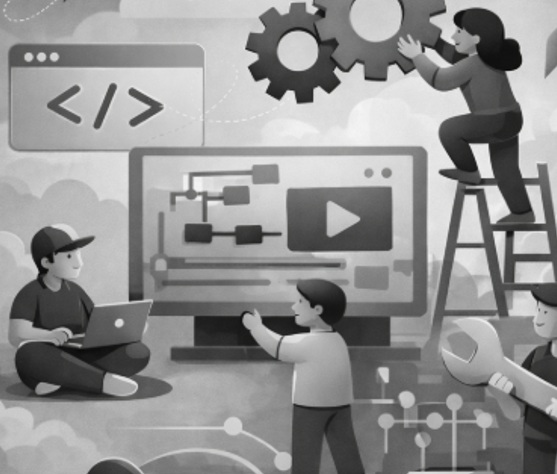
\includegraphics[width=0.8\textwidth]{FIGURAS/FIGURA_PARA_TEMPLATE.jpg}
% \caption*{\textbf{Source:} Adapted from \citeonline[p.~39]{latour2012we}}
% \label{fig:polos}
% \end{figure}





\section{Motivação}

A rejeição editorial precoce, conhecida na prática editorial como \textit{desk rejection}, é a recusa de um manuscrito antes de ser encaminhado à revisão de mérito. Uma observação central deste trabalho é que essa recusa raramente decorre de falhas científicas absolutas. Ela decorre, na maioria dos casos, da inadequação do manuscrito ao escopo, ao formato e às expectativas implícitas de uma trilha específica — em síntese, de um problema de conformidade, não de mérito. Um artigo metodologicamente sólido pode ser rejeitado na triagem simplesmente porque "não é o tipo de trabalho que aquela trilha publica".

Esse conhecimento — o que constitui um artigo bem-formado para determinada comunidade — é tácito, encontra-se distribuído nos artigos já aceitos e é adquirido lentamente, por imersão, ao longo da formação do pesquisador. É justamente o pesquisador em início de carreira quem menos o domina, e quem mais sofre suas consequências. A hipótese de trabalho que orienta esta proposta é a de que esse conhecimento tácito pode ser tornado explícito e computável a partir do corpus de artigos aceitos de uma conferência, e que um artefato pode usá-lo para orientar o autor antes da submissão.

\section{Problema e questão de pesquisa}

Identifica-se, assim, uma lacuna relacionada à compreensão de como agentes de IA podem ser estruturados para produzir avaliações contextualizadas ao gênero de uma comunidade científica, úteis à formação de novos pesquisadores. O problema de pesquisa consiste em investigar como modelar computacionalmente as convenções de gênero de uma trilha de conferência e utilizá-las para orientar autores, de modo a reduzir a rejeição editorial precoce.

Assim, o problema de pesquisa deste trabalho consiste em investigar como arquiteturas multiagentes baseadas em IA podem apoiar a avaliação sistemática de artigos científicos e contribuir para a qualificação das publicações em periódicos brasileiros.

A questão de pesquisa que orienta o estudo é:

\begin{quotation}
\noindent Agentes de IA podem contribuir para a redução da rejeição editorial a partir do corpus de artigos aceitos, e utilizá-las para produzir orientação acionável que apoie autores em início de carreira e reduza a incidência de rejeição editorial precoce?
\end{quotation}


\section{Objetivos}

O objetivo geral é projetar, construir e avaliar um artefato de software, um tutor baseado em agentes de IA que modele o gênero de uma trilha de conferência e verifique a conformidade de manuscritos a esse gênero, gerando orientação formativa. Como objetivos específicos, definem-se: 

\begin{itemize}
    \item (i) formular uma fundamentação teórica que articule a Teoria de Gêneros \cite{GenresOrgComm}, a análise de moves retóricos e a teoria de compiladores sob o método DSR
    \item (ii) especificar uma teoria de design para essa classe de artefatos, segundo a anatomia de \cite{DesignTheory}
    \item (iii) definir e implementar um método eficiente para extrair, de todo o corpus de uma conferência, a especificação de gênero de cada trilha
    \item (iv) implementar o protótipo aplicado ao SBSI e outras conferências do SOL (SBC OpenLib) \cite{solsbc}, integrando modelos locais e comerciais
    \item (v) avaliar empiricamente o artefato quanto à utilidade percebida, à validade dos diagnósticos e à concordância com avaliadores humanos.
\end{itemize}




\section{Contribuições esperadas}

Esperam-se três contribuições. 
\begin{itemize}
    \item A primeira, técnica, é o próprio artefato e o método de compilação do corpus de uma conferência em uma base de conhecimento de gênero. 

    \item A segunda, teórica, é uma teoria de design — no sentido de \cite{GenresOrgComm} %Gregor e Jones (2007) 
para artefatos de IA que apoiam a enculturação em gêneros acadêmicos, generalizável para além do SBSI. 

    \item A terceira, aplicada, é evidência empírica sobre o efeito do artefato na conformidade dos manuscritos e na percepção de utilidade por autores em formação, no contexto brasileiro.
\end{itemize}

% \section{Organização do documento}

% O Capítulo 2 apresenta a fundamentação teórica. O Capítulo 3 discute os trabalhos relacionados. O Capítulo 4 formula a solução proposta como uma teoria de design. O Capítulo 5 detalha o método de construção do artefato. O Capítulo 6 descreve o método de avaliação. O Capítulo 7 apresenta o cronograma e os resultados esperados. O Capítulo 8 traz as considerações parciais.
